\chapter{System and Model}
The cart pendulum system from \textit{Part 1} is used again. However, here in \textit{Part 2} an additional pendulum is mounted on the cart. The modification is discussed and a model for the changed system is developed in this chapter. The remaining of \textit{Part 2} is concerned with estimating parameters, developing a state estimator and ultimately stabilizing the two pendulums in upright position.

\section{System Addition}


\section{Model}
To model the twin pendulum system, consider the excessive coordinate convention in \autoref{fig:excessiveCoordinatesTwin} along with the generalized coordinates in the mechanical drawing, \autoref{fig:mechanicalDrawingTwin}.
\begin{figure}[H]
  \captionbox
  {
    Twin pendulum system in excessive coordinates.
    \label{fig:excessiveCoordinatesTwin}
  }
  {
    \hspace{-1cm}
    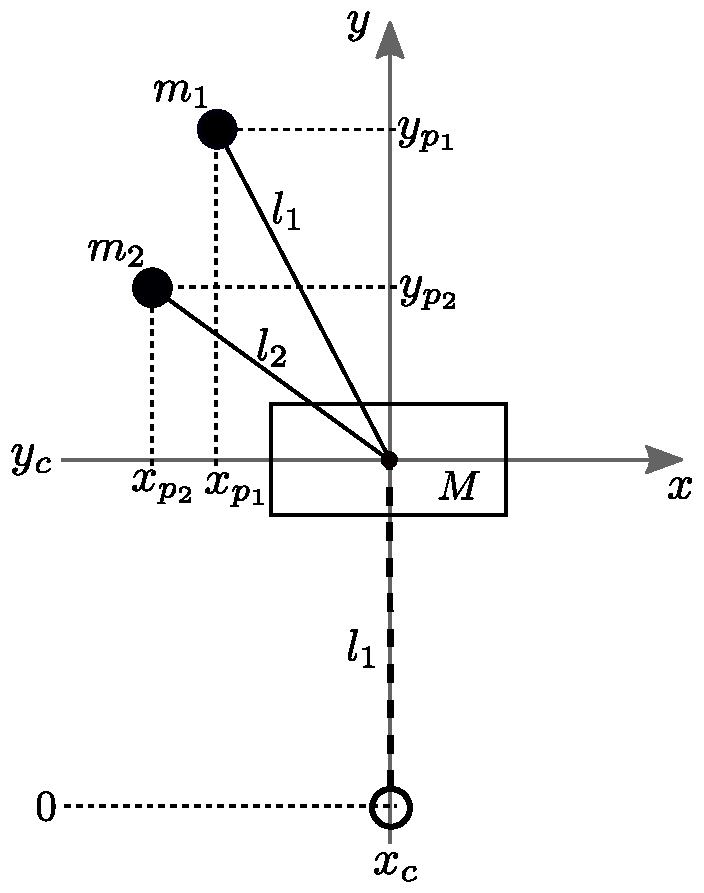
\includegraphics[width=.35\textwidth]{figures/excessiveCoordinatesTwin}
  }
  \hspace{40pt}
  \captionbox
  {
    Mechanical drawing of the system with the added pendulum in generalized coordinates.
    \label{fig:mechanicalDrawingTwin}
  }
  {
    \hspace{-1cm}
    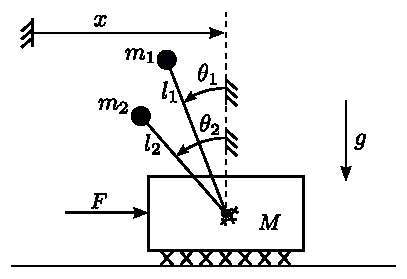
\includegraphics[width=.43\textwidth]{figures/mechanicalDrawingTwin}\vspace{1.2cm}
  }  
\end{figure}
%
The energy method is applied. First the potential and kinetic energies, in therms of excessive coordinates, is found,
\begin{align}
  U &= M g y_c + m_1 g y_{p_1} + m_2 g y_{p_2}  \label{eq:potentialEnergyTwin}  \\
  T &= \tfrac{1}{2} M \dot{x}_c^2 + \tfrac{1}{2} M \dot{y}_c^2 + \tfrac{1}{2} m_1 \dot{x}_{p_1}^2  + \tfrac{1}{2} m_1 \dot{y}_{p_1}^2 + \tfrac{1}{2} m_2 \dot{x}_{p_2}^2 + \tfrac{1}{2} m_2 \dot{y}_{p_2}^2 \label{eq:kineticEnergyTwin} \ \ \ .
\end{align}
%
The excessive coordinates and derivatives thereof are then expressed in therms of the generalized coordinates, using the conventions presented in \autoref{fig:excessiveCoordinatesTwin} and \ref{fig:mechanicalDrawingTwin},
\begin{align}
  \begin{cases}
    x_c &=  x  \\
    y_c &=  l_1  
  \end{cases} &
  \hspace{20pt}
  \begin{cases}
    x_{p_1} =  x   - l_1 \sin \theta_1 \\
    y_{p_1} =  l_1 + l_1 \cos \theta_1
  \end{cases}
  \hspace{10pt}
  \begin{cases}
    x_{p_2} =  x   - l_2 \sin \theta_2 \\
    y_{p_2} =  l_1 + l_2 \cos \theta_2
  \end{cases}
  \label{eq:excessiveToGeneralized} \\
  \begin{cases}
    \dot{x}_c &=  \dot{x}  \\
    \dot{y}_c &=  0  
  \end{cases} &
  \hspace{20pt}
  \begin{cases}
    \dot{x}_{p_1} =  \dot{x} - l_1 \sin \theta_1 \\
    \dot{y}_{p_1} =  -l_1 \sin \theta_1 \dot{\theta}_1
  \end{cases}
  \hspace{10pt}
  \begin{cases}
    \dot{x}_{p_2} = \dot{x} - l_2 \sin \theta_2 \\
    \dot{y}_{p_2} = -l_2 \sin \theta_2 \dot{\theta}_2
  \end{cases}  \ \ \ .
  \label{eq:excessiveToGeneralizedDerivatives}
\end{align}

Inserting \autoref{eq:excessiveToGeneralized} and \ref{eq:excessiveToGeneralizedDerivatives} into the energy equations, \autoref{eq:potentialEnergyTwin} and \ref{eq:kineticEnergyTwin}, yields,
%
\begin{align}
  U &= M g l_1 + m_1 g (l_1 + l_1 \cos \theta_1) + m_2 g (l_1 + l_2 \cos \theta_2)  \label{eq:potentialEnergyTwinGeneralized}  \\
  T &= \tfrac{1}{2} M \dot{x}^2 + \tfrac{1}{2} m_1 (\dot{x} - l_1 \sin \theta_1)^2  + \tfrac{1}{2} m_1 (-l_1 \sin \theta_1 \dot{\theta}_1)^2 + \nonumber \\
    &+ \tfrac{1}{2} m_2 (\dot{x} - l_2 \sin \theta_2)^2 + \tfrac{1}{2} m_2 (-l_2 \sin \theta_2 \dot{\theta}_2)^2 \label{eq:kineticEnergyTwinGeneralized} \ \ \ .
\end{align}
%
Proceeding to compute the Lagrangian,
\begin{align}
  \cal{L} &= T - U   \\ 
%  \cal{L} &= \tfrac{1}{2} M \dot{x}^2 + \tfrac{1}{2} m_1 (\dot{x} - l_1 \sin \theta_1)^2  + \tfrac{1}{2} m_1 (-l_1 \sin \theta_1 \dot{\theta}_1)^2  \\
%          &+ \tfrac{1}{2} m_2 (\dot{x} - l_2 \sin \theta_2)^2 + \tfrac{1}{2} m_2 (-l_2 \sin \theta_2 \dot{\theta}_2)^2 \\
%          &- M g l_1 - m_1 g (l_1 + l_1 \cos \theta_1) - m_2 g (l_1 + l_2 \cos \theta_2)) \\
  \cal{L} &= \tfrac{1}{2} M \dot{x}^2 + \tfrac{1}{2} m_1 ( \dot{x}^2 + l_1^2 \cos ^2 \theta_1 \dot{\theta}_1^2 - 2 \dot{x} l_1 \cos \theta_1 \dot{\theta}_1 ) + \tfrac{1}{2} m_1 l_1^2 \sin ^2 \theta_1 \dot{\theta}_1^2 + \nonumber \\
          &+ \tfrac{1}{2} m_2 ( \dot{x}^2 + l_2^2 \cos ^2 \theta_2 \dot{\theta}_2^2 - 2 \dot{x} l_2 \cos \theta_2 \dot{\theta}_2 ) + \tfrac{1}{2} m_2 l_2^2 \sin ^2 \theta_2 \dot{\theta}_2^2 - \nonumber \\
          &-(M + m_1 + m_2) g l_1 - m_1 g l_1 \cos \theta_1 - m_2 g l_2 \cos \theta_2 \\
  \cal{L} &= \tfrac{1}{2} (M + m_1 + m_2) \dot{x}^2 - ( m_1 l_1 \cos \theta_1 \dot{\theta}_1 + m_2 l_2 \cos \theta_2 \dot{\theta}_2 ) \dot{x} + \nonumber \\
          &+ \tfrac{1}{2} m_1 l_1^2 (\cos^2 \theta_1 + \sin^2 \theta_1)\dot{\theta}_1^2 + \tfrac{1}{2} m_2 l_2^2 (\cos^2 \theta_2 + \sin^2 \theta_2)\dot{\theta}_2^2 - \nonumber \\
          &- (M + m_1 + m_2)g l_1 - m_1 g l_1 \cos \theta_1 - m_2 g l_2 \cos \theta_2  \\
  \cal{L} &= \tfrac{1}{2} (M + m_1 + m_2) \dot{x}^2 - ( m_1 l_1 \cos \theta_1 \dot{\theta}_1 + m_2 l_2 \cos \theta_2 \dot{\theta}_2 ) \dot{x} + \tfrac{1}{2} m_1 l_1^2 \dot{\theta}_1^2 + \nonumber \\
          &+ \tfrac{1}{2} m_2 l_2^2 \dot{\theta}_2^2 - (M + m_1 + m_2)g l_1 - m_1 g l_1 \cos \theta_1 - m_2 g l_2 \cos \theta_2
  \ \ \ , 
  \label{eq:lagrangian}
\end{align}
and finally by using the Lagrange-d’Alembert Principle, \cite{RWisniewski}
\begin{align}
  \frac{d}{dt}  \frac{\partial \cal{L}}{\partial \dot{\vec{q}}} - \frac{\partial \cal{L}}{\partial \vec{q}}  &=  \vec{Q} \ \ \ ,
  \label{eq:energyMethodWithExternalForcesTwin}
\end{align}
\begin{align}
  \vec{q} &= 
  \begin{bmatrix}
    \theta_1    \\
    \theta_2    \\
    x
  \end{bmatrix} \ \ \ , \ \ \ 
  \vec{Q} =
  \begin{bmatrix}
    -b_{p_1,v} \dot{\theta}_1 - \tanh(\text{k}_\text{tanh}\dot{\theta}_1) b_{p_1,c}    \\
    -b_{p_2,v} \dot{\theta}_2 - \tanh(\text{k}_\text{tanh}\dot{\theta}_2) b_{p_2,c}    \\
    u - b_{c,v} \dot{x} - \tanh(\text{k}_\text{tanh}\dot{x}) b_{c,c}
  \end{bmatrix} \ \ \ .
  \label{eq:qAndQ_twin}
\end{align}
%
Note that, as in \textit{Part 1}, the control output is seen as the force on the cart directly, $u = F$, to avoid excessive notation. \autoref{eq:energyMethodWithExternalForcesTwin} is computed for each generalized coordinate starting with the first pendulum angle, $\theta_1$,
\begin{gather}
\frac{d}{dt}  \frac{\partial \cal{L}}{\partial \dot{\theta}_1} - \frac{\partial \cal{L}}{\partial \theta_1}  = Q_1 \\
m_1 l_1 \sin \theta_1 \dot{\theta}_1 \dot{x} - m_1 l_1 \cos \theta_1 \ddot{x} + m_1 l_1^2 \ddot{\theta}_1 - m_1 l_1 \sin \theta_1 \dot{\theta}_1 \dot{x} - m_1 g l_1 \sin \theta_1 = Q_1  \\
- m_1 l_1 \cos \theta_1 \ddot{x} + m_1 l_1^2 \ddot{\theta}_1 - m_1 g l_1 \sin \theta_1 = -b_{p_1,v} \dot{\theta}_1 - \tanh(\text{k}_\text{tanh}\dot{\theta}_1) b_{p_1,c}  \ \ \ ,
\label{eq:theta1Dynamics}
\end{gather}
similarly for the second pendulum angle, $\theta_2$,
\begin{gather}
- m_2 l_2 \cos \theta_2 \ddot{x} + m_2 l_2^2 \ddot{\theta}_2 - m_2 g l_2 \sin \theta_2 = -b_{p_2,v} \dot{\theta}_2 - \tanh(\text{k}_\text{tanh}\dot{\theta}_2) b_{p_2,c}  \ \ \ ,
\label{eq:theta2Dynamics}
\end{gather}
and finally for the cart position, $x$,
\begin{gather}
\frac{d}{dt}  \frac{\partial \cal{L}}{\partial \dot{x}} - \frac{\partial \cal{L}}{\partial x}  = Q_3 \\
(M + m_1 + m_2) \ddot{x} + m_1 l_1 \sin \theta_1 \dot{\theta}_1^2 - m_1 l_1 \cos \theta_1 \ddot{\theta}_1 + \nonumber \\
+ m_2 l_2 \sin \theta_2 \dot{\theta}_2^2 - m_2 l_2 \cos \theta_2 \ddot{\theta}_2 = u - b_{c,v} \dot{x} - \tanh(\text{k}_\text{tanh}\dot{x}) b_{c,c}  \ \ \ .
\label{eq:xDynamics}
\end{gather}
%
The final dynamic equations for the twin pendulum system are then,
%
\begingroup\makeatletter\def\f@size{10}\check@mathfonts
\def\maketag@@@#1{\hbox{\m@th\normalsize\normalfont#1}}%
\begin{gather}
- m_1 l_1 \cos \theta_1 \ddot{x} + m_1 l_1^2 \ddot{\theta}_1 - m_1 g l_1 \sin \theta_1 = Q_1 
\label{eq:theta1Dynamics1} \\
- m_2 l_2 \cos \theta_2 \ddot{x} + m_2 l_2^2 \ddot{\theta}_2 - m_2 g l_2 \sin \theta_2 = Q_2
\label{eq:theta2Dynamics1} \\
(M + m_1 + m_2) \ddot{x} + m_1 l_1 \sin \theta_1 \dot{\theta}_1^2 - m_1 l_1 \cos \theta_1 \ddot{\theta}_1 + m_2 l_2 \sin \theta_2 \dot{\theta}_2^2 - m_2 l_2 \cos \theta_2 \ddot{\theta}_2 = Q_3  \ \ \ , 
\label{eq:xDynamics1} \\ \nonumber
\end{gather}\endgroup \vspace{-44pt}

and arranged in following manner,
%
\begingroup\makeatletter\def\f@size{10}\check@mathfonts
\def\maketag@@@#1{\hbox{\m@th\normalsize\normalfont#1}}%
\begin{align}
  \begin{split}
    &
    \begin{bmatrix}
      m_1 l_1^2              & 0                       &  -m_1 l_1 \cos \theta_1 \\
      0                      & m_2 l_2^2               &  -m_2 l_2 \cos \theta_2\\
      -m_1 l_1 \cos \theta_1 & -m_2 l_2 \cos \theta_2  &  M + m_1 + m_2
    \end{bmatrix}
    \begin{bmatrix}
      \ddot{\theta}_1  \\
      \ddot{\theta}_2  \\
      \ddot{x}
    \end{bmatrix}
    +
    \begin{bmatrix}
    0  \\
    0  \\
    m_1 l_1 \sin \theta_1 \dot{\theta}_1^2 + m_2 l_2 \sin \theta_2 \dot{\theta}_2^2
    \end{bmatrix}
    +   \\
    &+
    \begin{bmatrix}
      -b_{p_1,v} \dot{\theta}_1 - \tanh(\text{k}_\text{tanh}\dot{\theta}_1) b_{p_1,c}    \\
      -b_{p_2,v} \dot{\theta}_2 - \tanh(\text{k}_\text{tanh}\dot{\theta}_2) b_{p_2,c}    \\
      -b_{c,v} \dot{x} - \tanh(\text{k}_\text{tanh}\dot{x}) b_{c,c}
    \end{bmatrix}
    +
    \begin{bmatrix}
      -m_1 g l_1 \sin \theta_1  \\
      -m_2 g l_2 \sin \theta_2  \\
      0
    \end{bmatrix}
    =
    \begin{bmatrix}
      0  \\
      0  \\
      u
    \end{bmatrix} \ \ \ , 
  \end{split}
  \label{eq:theta1Theta2Xdynamics} \\ \nonumber
\end{align}
\endgroup \vspace{-44pt}

the well known general form of an m-link robot is obtained, \cite{MWSpong, LSciavicco}
\begin{align}
\vec{M}(\vec{q})\vec{\ddot{q}} + \vec{C}(\vec{q},\vec{\dot{q}}) + \vec{B}(\vec{\dot{q}}) + \vec{G}(\vec{q}) &= \vec{F} \ \ \ , \hspace{3.3cm}
\end{align}
\begin{where}
  \va{ \vec{M}(\vec{q})  }{is the inertia matrix}                    {}
  \va{ \vec{C}(\vec{q},\vec{\dot{q}})  }{is the Coriolis and centrifugal effects}  {}
  \va{ \vec{B}(\vec{\dot{q}})          }{is the friction}                          {}
  \va{  \vec{G}(\vec{q})               }{is the force due to gravity}              {}
  \va{  \vec{F}                        }{is the input force vector \ \ \ .}        {}
\end{where}

Choosing states $ [\ x_1\ \ x_2\ \ x_3\ x_4\ \ x_5\ \ x_6\ ]^\mathrm{T} = [\ \theta_1\ \ \theta_2\ \ x\ \ \dot{\theta}_1\ \ \dot{\theta}_2\ \ \dot{x}\ ]^\mathrm{T} $ results in the nonlinear state space representation,
%
%\begingroup\makeatletter\def\f@size{10}\check@mathfonts
%\def\maketag@@@#1{\hbox{\m@th\normalsize\normalfont#1}}%
\begin{align}
  \begin{bmatrix}
    \dot{x_1} \\
    \dot{x_2} \\
    \dot{x_3} \\
    \dot{x_4} \\
    \dot{x_5} \\
    \dot{x_6}
  \end{bmatrix}
  &=
  \begin{bmatrix}
    x_4 \\
    x_5 \\
    x_6 \\
    \\
    \vec{M}^{-1}(x_1,x_2) ( \vec{F} - \vec{C}(x_1,x_2,x_4,x_5) - \vec{B}(x_4,x_5,x_6) - \vec{G}(x_1,x_2) ) \\
    \phantom{eq}
  \end{bmatrix}
  \label{eq:nonlinearStateSpaceTwin} \ \ \ . %\\ \nonumber
\end{align}
%\endgroup \vspace{-44pt}
%















